\documentclass[a4paper,11pt]{article}
\usepackage{fullpage}
\usepackage[colorlinks=true]{hyperref}
\usepackage{cleveref}
\usepackage{algorithm}
\usepackage{algpseudocode}
\usepackage{amssymb}
\usepackage{amsmath}
\usepackage{fancyhdr}
\usepackage{verbatim}
\usepackage{lmodern}
\usepackage{listings}
\usepackage{graphicx}
\usepackage{booktabs}
\usepackage{caption}
\usepackage{color}
\usepackage[toc]{glossaries}

\setlength{\headheight}{26pt}
\setlength{\headsep}{0.2in}

\definecolor{gray}{rgb}{0.5, 0.5, 0.5}
\crefname{figure}{figure}{figures}

\lstset{
    language=Python,
    basicstyle=\footnotesize,
    numbers=left,
    numberstyle=\scriptsize\color{gray},
    stepnumber=1,
    numbersep=5pt,
    backgroundcolor=\color{white},
    showspaces=false,
    showstringspaces=false,
    rulecolor=\black,
    tabsize=4,
    captionpos=t,
    breaklines=true,
    keywordstyle=\color{black},
    commentstyle=\color{black},
    stringstyle=\color{black}
}

\title{OpenCUDA+MPI\\
       A Framework for Heterogeneous GP-GPU Distribute Computing}
\date{\today}
\author{Kenny Ballou\\
        Nilab Mohammad-Mousa\\
        College of Engineering --- Department of Computer Science\\
        Boise State University\\
        Alark Joshi, Ph. D}
\lhead{\fancyplain{}{Student Research Initiative 2013\\
                     Progress Report}}
\pagestyle{empty}
\makeglossaries{}
\graphicspath{{../figures/}}
\begin{document}
\begin{titlepage}
\begin{center}

\textsc{\LARGE OpenCUDA+MPI}\\[1.5cm]
\textsc{\Large A Framework for Heterogeneous
               GP-GPU Distributed Computing}\\[1.5cm]

Kenny Ballou\\
Nilab Mohammad Mousa\\
College of Engineering -- Department of Computer Science\\
Boise State University\\
Alark Joshi, Ph.D\\
\vfill
\end{center}
\end{titlepage}

% vim: syntax=tex:
\newacronym{api}{API}{Application Programmable Interface}
\newacronym{boinc}{BOINC}{Berkeley Open Infrastructure for Network
                          Computputing}
\newacronym{cpu}{CPU}{Centeral Processing Unit}
\newacronym{cuda}{CUDA}{Compute Unified Device Architecture}
\newacronym{gpu}{GPU}{Graphics Processing Unit}
\newacronym{gpgpu}{GP-GPU}{General Purpose \Gls{gpu}}
\newacronym{io}{I/O}{Input/ Output}
\newacronym{mpi}{MPI}{Message Passing Interface}
\newacronym{p3m}{P3M}{Particle-Particle, Particle-Mesh}
\newacronym{pvm}{PVM}{Parallel Virtual Machine}
\newacronym{rdma}{RDMA}{Remote Direct Memory Access}
\newacronym{torque}{TORQUE}{Terascale Open-Source Resource and QUEue Manager}
\newglossaryentry{cluster}
{
    name=cluster,
    description={A collection of computers networked together, typically with
    the goal of combining computational power}
}
\newglossaryentry{cpu_time}
{
    name=\gls{cpu} time,
    description={time (typically in seconds) spent executing the process}
}
\newglossaryentry{ib}
{
    name=Infiniband,
    description={a networking fabric specification that defines a connection
    between compute nodes}
}
\newglossaryentry{node}
{
    name=node,
    description={a computer, member of a \gls{cluster}}
}
\newglossaryentry{real_time}
{
    name=real time,
    description={Elapsed time excuting; synonomous of \gls{wall_time}}
}
\newglossaryentry{slot}
{
    name=slot,
    description={process space on a \gls{node}, typically equal to the number
    of logical \gls{cpu} cores on the node}
}
\newglossaryentry{sys_time}
{
    name=system time,
    description={similar to \gls{sys_time}, the amount of time the ``system''
    was executing}
}
\newglossaryentry{user_time}
{
    name=user time,
    description={similar to \gls{cpu_time}, the amount of time ``user'' code
    was executing}
}
\newglossaryentry{wall_time}
{
    name=wall time,
    description={all elapsed time (typically in seconds) that passes from start
    to finish of a program}
}

\nocite{*}
\thispagestyle{fancy}
\begin{abstract}
The introduction and rise of General Purpose Graphics Computing has
significantly impacted parallel and high-performance computing. It has
introduced challenges when it comes to distributed computing with GPUs. Current
solutions target specifics: specific hardware, specific network topology, a
specific level of processing. Those restrictions on GPU computing limit
scientists and researchers in various ways. The goal of OpenCUDA+MPI project is
to develop a framework that allows researchers and scientists to write a
general algorithm without the overhead of worrying about the specifics of the
hardware and the cluster it will run against while taking full advantage of
parallel and distributed computing on GPUs. As work toward the solution
continues to progress, we have proven the need for the framework and expect to
find the framework enables scientists to focus on their research.
\end{abstract}

\textbf{Keywords:} Parallel Computing, Distributed Computing, General Purpose
Graphics Processing, High-Performance Computing, Scientific Computing,
Frameworks, Software Libraries
\newpage{}
% vim: syntax=tex:
\section{Topic}

Increasingly, \Glspl{gpu} are being used for general purpose computation
(\gls{gpgpu}). They have significantly altered the way high-performance
computing tasks can be performed today. To accelerate general-purpose
scientific applications, computationally intensive portions of the application
are passed to \glspl{gpu}. Once the \gls{gpu} has completed its task it sends
the result back to the \Gls{cpu} where the application code is running. This
process can make applications run noticeably faster.

Scientific applications require a large number of floating point number
operations, \Glspl{cpu} are not sufficient to carry out such computationally
intensive tasks. \glspl{cpu} are responsible for prioritization and execution
of every instruction. Generally, a processor is described by the number of
execution cores it owns. Modern Central Processing Unit have eight cores while
\Glspl{gpu} have hundreds or more cores. More cores grant \glspl{gpu} the
ability to perform more tasks at the same time.

In computer architecture there are two main ways of processing: serial and
parallel. \Glspl{cpu} consist of a small number of cores (microprocessors) that
are best at processing serial data. On the other hand, \glspl{gpu} consist of
thousands of cores that are designed for processing parallel data. Given a
program, we can run the parallel portions of the code on \glspl{gpu} while the
serial portions run on the \gls{cpu}\@. The programmable \gls{gpu} has evolved
into a highly parallel, multithreaded, many core processor with tremendous
computational power. \Gls{cuda} is an architecture for utilizing and
distributing computational tasks onto a computer's \glspl{gpu}. As a parallel
computing platform and programming model, \gls{cuda} utilizes the power of
\gls{gpu} to achieve dramatic increases in computing performance
\cite{website:cudaCProgrammingGuide}. This fact is well illustrated in
Figure 1 Floating-Point Operations per Second for the \gls{cpu} and
\gls{gpu}.\\

\begin{figure}[htb]
\centering
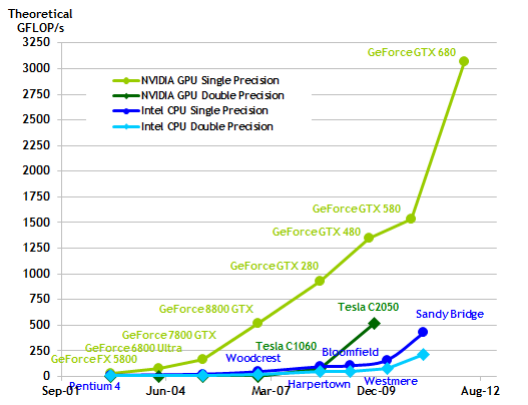
\includegraphics[scale=0.75]{img/floatingPoint.png}
\caption{Floating-Point Operations per Second for the \gls{cpu} and
         \gls{gpu} \cite{website:cudaCProgrammingGuide}}
\end{figure}

Today, more than one million \gls{cuda}-enabled \glspl{gpu} are used by
software developers, scientists and researchers in order to obtained a large
performance gain in wide-ranging applications
\cite{website:cudaCProgrammingGuide}. A major challenge remains in being
able to seamlessly integrate multiple workstations to further parallelize the
computational tasks \cite{hadri2010identifying} \cite{hindman2009common}.
Current approaches provide the ability to parallelize tasks, but they are less
focused on optimally utilizing the varied capabilities of heterogeneous
graphics cards in a cluster of workstations (across many computer nodes).

We propose to create a framework for using both \Gls{mpi} and \gls{cuda} on a
cluster of computers to dynamically and easily assign computationally intensive
tasks to the machines participating in the cluster.  \Gls{mpi} is a popularly
used standardized interface for communication among a group of computers. It
facilitates the passing of messages between the nodes in the cluster.

Our framework will be easy to use on a heterogeneous cluster of computers, each
containing a \Gls{cuda}-capable \gls{gpu}\@. The framework will optimize the
scheduling of low-level computational tasks based on the capabilities of the
varied \glspl{gpu} in the cluster. The framework will provide the system
administrator with the ability to easily configure it to allow optimal use of
the individual \glspl{gpu}. Overall, the goal is to create a framework that is
simple and easy to use, facilitating the combination of two powerful means of
computing to further increase the throughput and overall computing power of a
cluster.

We plan to evaluate the efficacy of our framework on the problem of vessel
extraction. Currently, we use a single \gls{gpu} to extract vascular structures
from a CT angiography scan which is computationally intensive
\cite{erdt2008automatic}. Using the framework to accelerate the computational
task will provide us with key insights on its usability.

% vim: syntax=tex:
\section{Significance}

\texttt{CUDA+MPI} will serve to better utilization of existing computing
resources. In other words, it will give us high compute power at low cost. Many
personal computers have a \gls{cuda} graphics card. It is more cost effective
to build a cluster of multiple computers than to purchase a supercomputer to
perform high performance computing. The reason for the low costs stem from the
fact that clusters are built of components which are sold in high volumes
\cite{erdt2008automatic}. \texttt{CUDA+MPI} will have the advantage of handling
heterogeneous distributed computing. In other words, \texttt{CUDA+MPI} avoids
hardware limitations. All the computers participating in the cluster do not
need to have the same model of \gls{cuda}-enabled \gls{gpu} cards. This will
also give us the freedom to easily add new nodes to the cluster as needed.

Since \texttt{CUDA+MPI} will operate in a heterogeneous cluster it will manage
the job requests from the user to be run on a heterogeneous cluster of
\gls{gpu}-capable computers. In order to decide job priority, amount of work
and availability of devices will be considered. In addition to improved
performance, the proposed framework will grant researchers and scientists the
assurance that the heterogeneous cluster will be optimized for computing
without requiring extra effort and thought.

% vim: syntax=tex:
\section{Related Works}

Current approaches to accelerating research computations and engineering
applications include parallel computing and distributed computing. A parallel
system is when several processing elements work simultaneously to solve a
problem faster. The primary consideration is elapsed time, not throughput or
sharing of resources at remote locations. A distributed system is a collection
of independent computers that appears to its users as a single coherent system.
In distributed computing the data is split into smaller parts and subsequently
spread across the system. The result is then collected and outputted. Summary
of current solutions are listed in \cref{tab:relatedProjects} below followed by
detailed description of every entry.\\

\begin{table}[htb]
\centering
\begin{tabular}{ll}
\toprule{}
\textbf{Project}   & \textbf{Description} \\
\midrule{}
\texttt{Hadoop}    & Distributed computation framework
                     \cite{website:Hadoop-Wiki} \cite{website:Apache-Hadoop}
                     \cite{shvachko2011apache}\\
\midrule{}
\texttt{BOINC}     & Volunteer and grid computing project distributed
                     \cite{anderson2004boinc} \\
\midrule{}
\texttt{GPUDirect} & \gls{gpu}-to-\gls{gpu} framework for parallel computing
                     \cite{website:youtube_gpudirect} \\
\midrule{}
\texttt{MPI}       & Message-passing system for parallel computations
                     \cite{website:MPI-Tutorial} \cite{website:mpi-4-python} \\
\midrule{}
\texttt{PVM}       & Distributed environment and message passing system
                     \cite{website:Computer-Science-and-Division} \\
\bottomrule{}
\end{tabular}
\caption{Summary of Current Approaches and Projects}
\label{tab:relatedProjects}
\end{table}

\subsection{Hadoop}

Hadoop provides a distributed file system and a framework
for the analysis and transformation of very large data sets using the MapReduce
paradigm \cite{website:Apache-Hadoop} \cite{website:Apress} \cite{dias2011hpc}
\cite{dean2001mapreduce}. An important characteristic of Hadoop is the
partitioning of data and computation across many (thousands) of hosts (nodes),
and executing application computations in parallel close to their data
\cite{shvachko2011apache}. The MapReduce \cite{luo2011hierarchical}
\cite{website:Hadoop-Wiki-map} paradigm which Hadoop implements is
characterized by dividing the application into many small fragments of work,
each of which may be executed or re-executed on any node in the cluster. The
worker node processes the smaller problem, and passes the answer back to its
master node. The answers to the subproblems are then combined to form the
output. Hadoop is popular model for distributed computations, however, it is
does not integrate with \gls{cuda}-enabled \glspl{gpu}.

\subsection{BOINC}

The \Gls{boinc} is an open source middleware system for volunteer and grid
computing. The general public can contribute to today's computing power by
donating their personal computer's disk space and some percentage of \gls{cpu}
and \gls{gpu} processing. In other words, \gls{boinc} is software that can use
the unused \gls{cpu} and \gls{gpu} cycles on a computer to do scientific
computing \cite{anderson2004boinc}. The \gls{boinc} project allows for
distributed computing using hundreds of millions of personal computers and game
consoles belonging to the general public. This paradigm enables previously
in-feasible research and scientific super-computing. The framework requires
that individuals are connected to the Internet and is supported by various
operating systems, including Microsoft Windows, Mac OS X and various Unix-like
systems. Although \Gls{boinc} may not seem relevant to our framework, it
represents a different paradigm in the realm of parallel and distributed
computing that our framework could use as an example for certain problems.

\subsection{GPUDirect}

Currently \gls{gpu} based clusters are becoming more popular.
\texttt{GPUDirect} is a \gls{gpu} \gls{rdma} communication specification using
\gls{ib}. \texttt{GPUDirect} allows for multiple \glspl{gpu} to communicate
with each other directly by giving \glspl{gpu} the ability to directly copy
memory to another \gls{gpu} \cite{website:youtube_gpudirect}. Prior to
GPUDirect, \gls{gpu}-to-\gls{gpu} communication involved the \gls{cpu}.
\texttt{GPUDirect} performance gain exceed \gls{cpu} solutions. Direct
\gls{gpu}-to-\gls{gpu} communication is less computationally expensive since
less messages will be sent and received via the host server. An issue with
\texttt{GPUDirect} is that it requires specific hardware.

\subsection{MPI}

\Gls{mpi} is the dominant message passing programming paradigm for clusters
\cite{website:Message-Passing-Interface-Forum}
\cite{website:Message-Passing-Interface}. \gls{mpi} is a standardized and
portable message-passing system that functions on a wide variety of parallel
computers. Although the standard \gls{mpi} defines the syntax and semantics of
a core of library routines in the \texttt{C} programming language, many other
languages offer \gls{api} call into \gls{mpi}. \texttt{OpenCUDA+MPI} builds
upon this model due to the fact that \gls{mpi} is the dominant model used in
high-performance computing \cite{sur2006high}. \Gls{mpi} has been implemented
for almost every distributed memory architecture and is optimized for the
hardware on which it runs.

\subsection{PVM}

\Gls{pvm} is a software tool for parallel networking of computers. It is
designed to allow a network of heterogeneous Unix and/or Windows machines to be
used as a single distributed parallel processor. Thus, large computational
problems can be solved more cost effectively by using the aggregate power and
memory of many computers. \gls{pvm} enables users to exploit their existing
computer hardware to solve much larger problems at less additional cost
\cite{website:Computer-Science-and-Division}. \gls{pvm} was a step towards
modern trends in distributed processing and grid computing but has, since the
mid-1990s, largely been supplanted by the much more successful \gls{mpi}
standard for message passing on parallel machines.

\subsection{CUDA+MPI}

The proposed \texttt{CUDA+MPI} framework will take advantage of both \gls{mpi}
and \gls{cuda} to perform computations on \gls{gpu} cards of computers
participating in the cluster. \texttt{CUDA+MPI}'s goal is to allow a collection
of heterogeneous computers each containing a \gls{cuda}-capable \gls{gpu} to be
used as a coherent and flexible concurrent computational resource.

% vim: syntax=tex:
\section{Methodology}

Our framework will be developed using a number of tools and will also build
upon a few already developed and mature software libraries. Overall, we plan to
use the \texttt{Python} programming language, \gls{mpi} for cross process
communication, and \gls{cuda} for graphics computing.

\subsection{Python}

We will use \texttt{Python} programming language because of its ease of
development and plethora of existing libraries such as \texttt{mpi4py} and
\texttt{pyCUDA}. \texttt{Python} also adds some advantages when it comes to
usability when needing more performance. For example, if we discover a need
for certain aspects of the project to be tuned or otherwise run faster, we can
easily switch to C or C++ and write sections of the program in a (more
performant) native language.

\subsection{MPI}

Currently our cluster consists of 16 computers provided to our research lab by
the Computer Science department of Boise State University. We will use
\gls{mpi} because it has established itself as the de-facto interface for cross
process communication \cite{website:MPI-Tutorial}. To allow for interfacing
with \texttt{Python} \cite{website:mpi-4-python}, we will use \texttt{mpi4py}
because of the library's maturity and implementation completeness.

\subsection{CUDA}

We will be using \gls{cuda}, and in particular, \texttt{pyCUDA}, because of
existing knowledge of the library/ framework and also because it is a well
established library for \gls{gpu} computing.

\subsection{\texttt{OpenCUDA+MPI}}

Our frameworks' goal is to make accessible the power of \gls{cluster} computing
without necessarily knowing in-depth the complexities of inter-computer related
communication. Further, in doing so, we would like to expose functionality that
may not be available even in more established \gls{cluster} libraries and
frameworks. Namely, facilities for debugging and profiling.

\subsection{Testing}

To evaluate the efficacy and accuracy of our framework several tests will be
executed. As previously mentioned one of the first algorithms to be tested will
be the problem of vessel extraction. Accurately extracting vascular structures
from a Computerized Tomographic angiography--also called CT angiography
scans--is important for creating oncologic surgery planning tools as well as
medical visualization applications \cite{erdt2008automatic}.  Currently, we use
a single \gls{gpu} to extract vascular structures from a CT angiography scan,
which is computationally intensive.

The following test programs will be developed as time allows:

\begin{itemize}
    \item N-Body Simulation
    \item Prime Number Searching
\end{itemize}

Every test program will be evaluated in three categories: \gls{cpu}-only,
\gls{cuda}-only, \gls{cuda} and \gls{mpi} and \texttt{OpenCUDA+MPI}. Having all
of the prior solutions that do \emph{not} use the framework provides a baseline
time comparison and provide immense insights into the pains and difficulties we
are actually attempting to solve.

% vim: syntax=tex:
\section{Results}

\subsection{Vector Summation}

Our first developed test program was a $ 10 $ billion element wise vector
summation problem. This is a simple and, as we will see, a bad example of using
a cluster to speed up the computational time required. Although we did see a
increase in performance, the cost of \gls{io} far out weighs the benefit.
Specifically, to do the computation on one machine (one \gls{cpu}), it took a
\gls{wall_time} of $254$ seconds (about $4$ minutes) and a \gls{cpu_time} of
$13.7$ seconds.  Further, to do the computation using a single \gls{gpu} took
about $4172$ seconds (\gls{wall_time}) or about $70$ minutes, $13.83$ seconds
(\gls{cpu_time}) while the computing the summation of the cluster took about
$3177$ seconds (\gls{wall_time}) or about $50$ minutes, $10.51$ seconds
(\gls{cpu_time}). Our \gls{cpu} only implementation took the least amount of
elapsed time, it took the second longest \gls{cpu_time}. Our \gls{cuda} only
implementation took the longest in both \gls{wall_time} and \gls{cpu_time} and
our cluster implementation was shortest \gls{cpu_time} but seconds longest
elapsed time. The benefit of saving an upwards of $3.3$ seconds is not worth
the extra incurred cost of $2923$ seconds. Not so surprisingly though, running
the vector summation problem over the cluster \emph{without} using \gls{cuda}
does increase the overall elapsed time of the problem; namely, it took $226$
seconds \gls{wall_time} (currently the correct \gls{cpu_time} is unable to be
collected). Further, increasing the number of nodes part of the program's pool,
decreases the \gls{wall_time} for each node.

\begin{table}[htb]
\centering{}
\begin{tabular}{lcc}
\toprule{}
\textbf{Method} & \textbf{Time (s)} & \textbf{Total Time (s)} \\
\midrule{}
CPU Only & 13.7 & 254.13 \\
\midrule{}
CUDA (Single \Gls{node}) & 13.83 & 4172 \\
\midrule{}
MPI + CUDA (7 \glspl{node}) & 10.51 & (average) 3177 \\
\midrule{}
MPI (7 \glspl{node}) & & (average) 226  \\
\midrule{}
MPI (16 \glspl{slot}) & & (average) 149 \\
\bottomrule{}
\end{tabular}
\caption{Computational Timing Comparison of $ 10^9 $ element wise vector
summation}
\end{table}

\subsection{N-Body Problem}

We have several sizes of the \texttt{N-Body} problem that we tested with:
$2,001$ particles, $20,000$ particles, $200,000$ particles, $2,000,000$, and
$20,000,000$ particles.\\

The computational times are for only one time step. The method for computing
the gravitational potential is an adaptation of the \gls{p3m} method. The
benefit of using this method is we are able to nicely distribute the problem
over the \gls{cluster} and / or over a \gls{gpu} (because of memory
limitations) while maintaining a respectable accuracy for close body
interactions. Further, if a grid contains more bodies than a specified
threshold (in our case $200,000$), we can further sub-divide the grid to
improve performance and maintain accuracy still.\\

There are other algorithms for computing \texttt{N-Body} problems on the
\gls{cpu} that are quite efficient, notably, the Barnes-Hut Tree
algorithm\cite{barneshut1986}; however, using it would distort and confound the
comparisons between \gls{cpu}, \gls{gpu}, and \gls{cluster} implementations,
not to mention the complexities of implementing such an algorithm on
\glspl{gpu} and over a \gls{cluster}.

\subsubsection{N-Body --- CPU}

In \gls{cpu} tests, we were only able to complete several of the problem sizes;
the larger sizes are infeasible. Notably, the smaller sizes were computed in a
relatively respectable amount of time. While the bigger sizes were time
consuming, not even attempted, or aborted. For example, the 2 million body
problem was aborted after running for about 2 weeks.

\begin{table}[htb]
\centering{}
\begin{tabular}{lccc}
\toprule{}
\textbf{Size} & \textbf{User (seconds)} &
\textbf{Sys (seconds)} & \textbf{Real (seconds)} \\
\midrule{}
2001          & 28.81   & 0.02    & 30.77   \\
\midrule{}
20000         & 2382.40 & 2.27    & 2393    \\
\midrule{}
200000        & 113983  & 34.45   & 114349  \\
\midrule{}
2 million     & aborted & aborted & aborted \\
\midrule{}
20 million    & N/A     & N/A     & N/A     \\
\bottomrule{}
\end{tabular}
\caption{\gls{cpu} N-Body simulation using particle-particle method}
\label{tab:cpu_nbody}
\end{table}

\subsubsection{N-Body --- GPU}

As noted above, the \gls{gpu} (\gls{cuda}) implementation uses the same
computational method (\gls{p3m}). Using the \gls{gpu}, we were able to compute
the $ 20,000,000 $ size problem and may be able to compute larger sets within a
\emph{reasonable} amount of time. See \cref{tab:gpu_nbody} for a breakdown of
the running times.

\begin{table}[htb]
\centering{}
\begin{tabular}{lccc}
\toprule{}
\textbf{Size} & \textbf{User (seconds)} &
\textbf{Sys (seconds)} & \textbf{Real (seconds)} \\
\midrule{}
2001          & 10.08   & 1.52    & 14.14  \\
\midrule{}
20000         & 22.30   & 2.46    & 26.82  \\
\midrule{}
200000        & 44.63   & 4.84    & 52.86  \\
\midrule{}
2 million     & 186.59  & 21.23   & 217.60 \\
\midrule{}
20 million    & 1289.24 & 159.29  & 1510   \\
\bottomrule{}
\end{tabular}
\caption{Single \gls{gpu} (\gls{cuda}) N-Body simulation using \gls{p3m}
method}
\label{tab:gpu_nbody}
\end{table}

\subsubsection{N-Body --- 16 Node Cluster}

Similar to the other solutions, we are still using the \gls{p3m} method for
computing a single time step of the N-Body problem. Over 16 nodes, we were able
to see drastic improvements over \gls{cpu} and \gls{cuda} implementations.
Notably, in the $20,000$ problem size, the \gls{cluster} did nearly $19044\%$
better than the \gls{cpu} and about $115\%$ better than a single \gls{gpu}.
Further, in the $200,000$ problem size, we see the \gls{cluster} did about
$535,743\%$ better versus \gls{cpu} and about $148\%$ better versus \gls{gpu}.
See \cref{tab:cudampi_nbody} for times of each problem size.

\begin{table}[htb]
\centering{}
\begin{tabular}{lccc}
\toprule{}
\textbf{Size} & \textbf{User (seconds)} &
\textbf{Sys (seconds)} & \textbf{Real (seconds)} \\
\midrule{}
2001          & N/A     & N/A      & N/A     \\
\midrule{}
20000         & 0.17    & 0.032    & 12.50   \\
\midrule{}
200000        & 0.147   & 0.028    & 21.34   \\
\midrule{}
2 million     & 0.15    & 0.025    & 97.76   \\
\midrule{}
20 million    & 0.15    & 0.06     & 950.045 \\
\bottomrule{}
\end{tabular}
\caption{16 node \gls{cluster} N-Body simulation using \gls{p3m} method}
\label{tab:cudampi_nbody}
\end{table}

% vim: syntax=tex:
\section{Conclusions}

We have developed some baseline test solutions to a few problems. From the
baseline solutions, we can easily tell there are significant performance
increases from parallelizing code. However, there is still a complexity cost.
The goal of \texttt{OpenCUDA+MPI} is to limit this complexity cost and from our
really early versions of the framework, the outlook of being able to do just
that looks very good.

\subsection{Future Work}

Work is continuing to progress on the development of the framework, but an
early alpha version is nearly complete. As we continue to develop the
framework, there are a few objectives we would like to achieve. Namely, we
would like to add better debugging and profiling functionality, expose
\gls{cuda} device initialization to the user, add automatic and/ or
configurable checkpointing, and finish node configuration and administrative
tasks.

\appendix
%% vim: syntax=tex:
\section{Appendix}

\subsection{Algorithms}

\begin{algorithm}
\begin{algorithmic}
\Function{Master}{$size,world\_size$}
    \Comment{Split data as appropriate and send to nodes}
    \State{$card\_max \gets query\_max\_mem()$}
    \State{$M \gets floor((N + card\_max - 1) / card\_max)$}
    \State{$m \gets floor((M + world\_size - 1) / world\_size)$}
    \ForAll{$r < world\_size$}
        \State{$slice\_low \gets (r * 2 + i) * card\_max$}
        \State{$slice\_high \gets (r * 2 + m) * card\_max$}
        \State{Send indices from low to high to node of rank $r$}
    \EndFor{}
\EndFunction{}
\Function{Minion}{$data,user\_fn$}
    \Comment{Receive Indices and Compute Results using user function}
    \State{$slice\_low \gets recv()$}
    \State{$slice\_high \gets recv()$}
    \State{$results \gets user\_fn(data[slice\_low:slice\_high])$}
    \State{Send back results or write them to disk}
\EndFunction{}
\end{algorithmic}
\label{alg:ocmf}
\caption{\texttt{OpenCUDA+MPI} Framework Pseudo Code}
\end{algorithm}

\begin{algorithm}
\begin{algorithmic}
\Function{main}{$rank$}
    \If{$rank == 0$} \State{$master(\dots{})$}
    \Else \State{$minion(\dots{})$}
    \EndIf{}
\EndFunction{}
\end{algorithmic}
\label{alg:run_code}
\caption{Combining the framework with user code}
\end{algorithm}

% vim: syntax=tex:
\section{Reference}
\renewcommand{\refname}{}
\bibliographystyle{plain}
\bibliography{references}

% vim: syntax=tex:
\section{Acknowledgements}

We would like to take this opportunity to thank everyone that helped and made
this project a possibility. Thanks to the Student Research Initiative
Fellowship for providing the motivation and funding. Lastly (and certainly not
least), a special thanks to our mentor, Alark Joshi, PhD., giving us the
high-level guidance and inspiration when it mattered most.

\printglossaries{}
\end{document}
